\subsection{From random inputs to a distribution}
A generator $g_w$ transforms a random input $Y\in\RR^r$ into an image $X=g_w(Y)\in\RR^d$. The input law $\eta$, for instance a standard Gaussian, is chosen in advance. The output law is the pushforward $\mu_w=(g_w)_\#\eta$. This notation describes how probability mass is redistributed by the network. A generator is a learned transformation, not generally the inverse of a classifier.

\begin{figure}[htbp]\centering
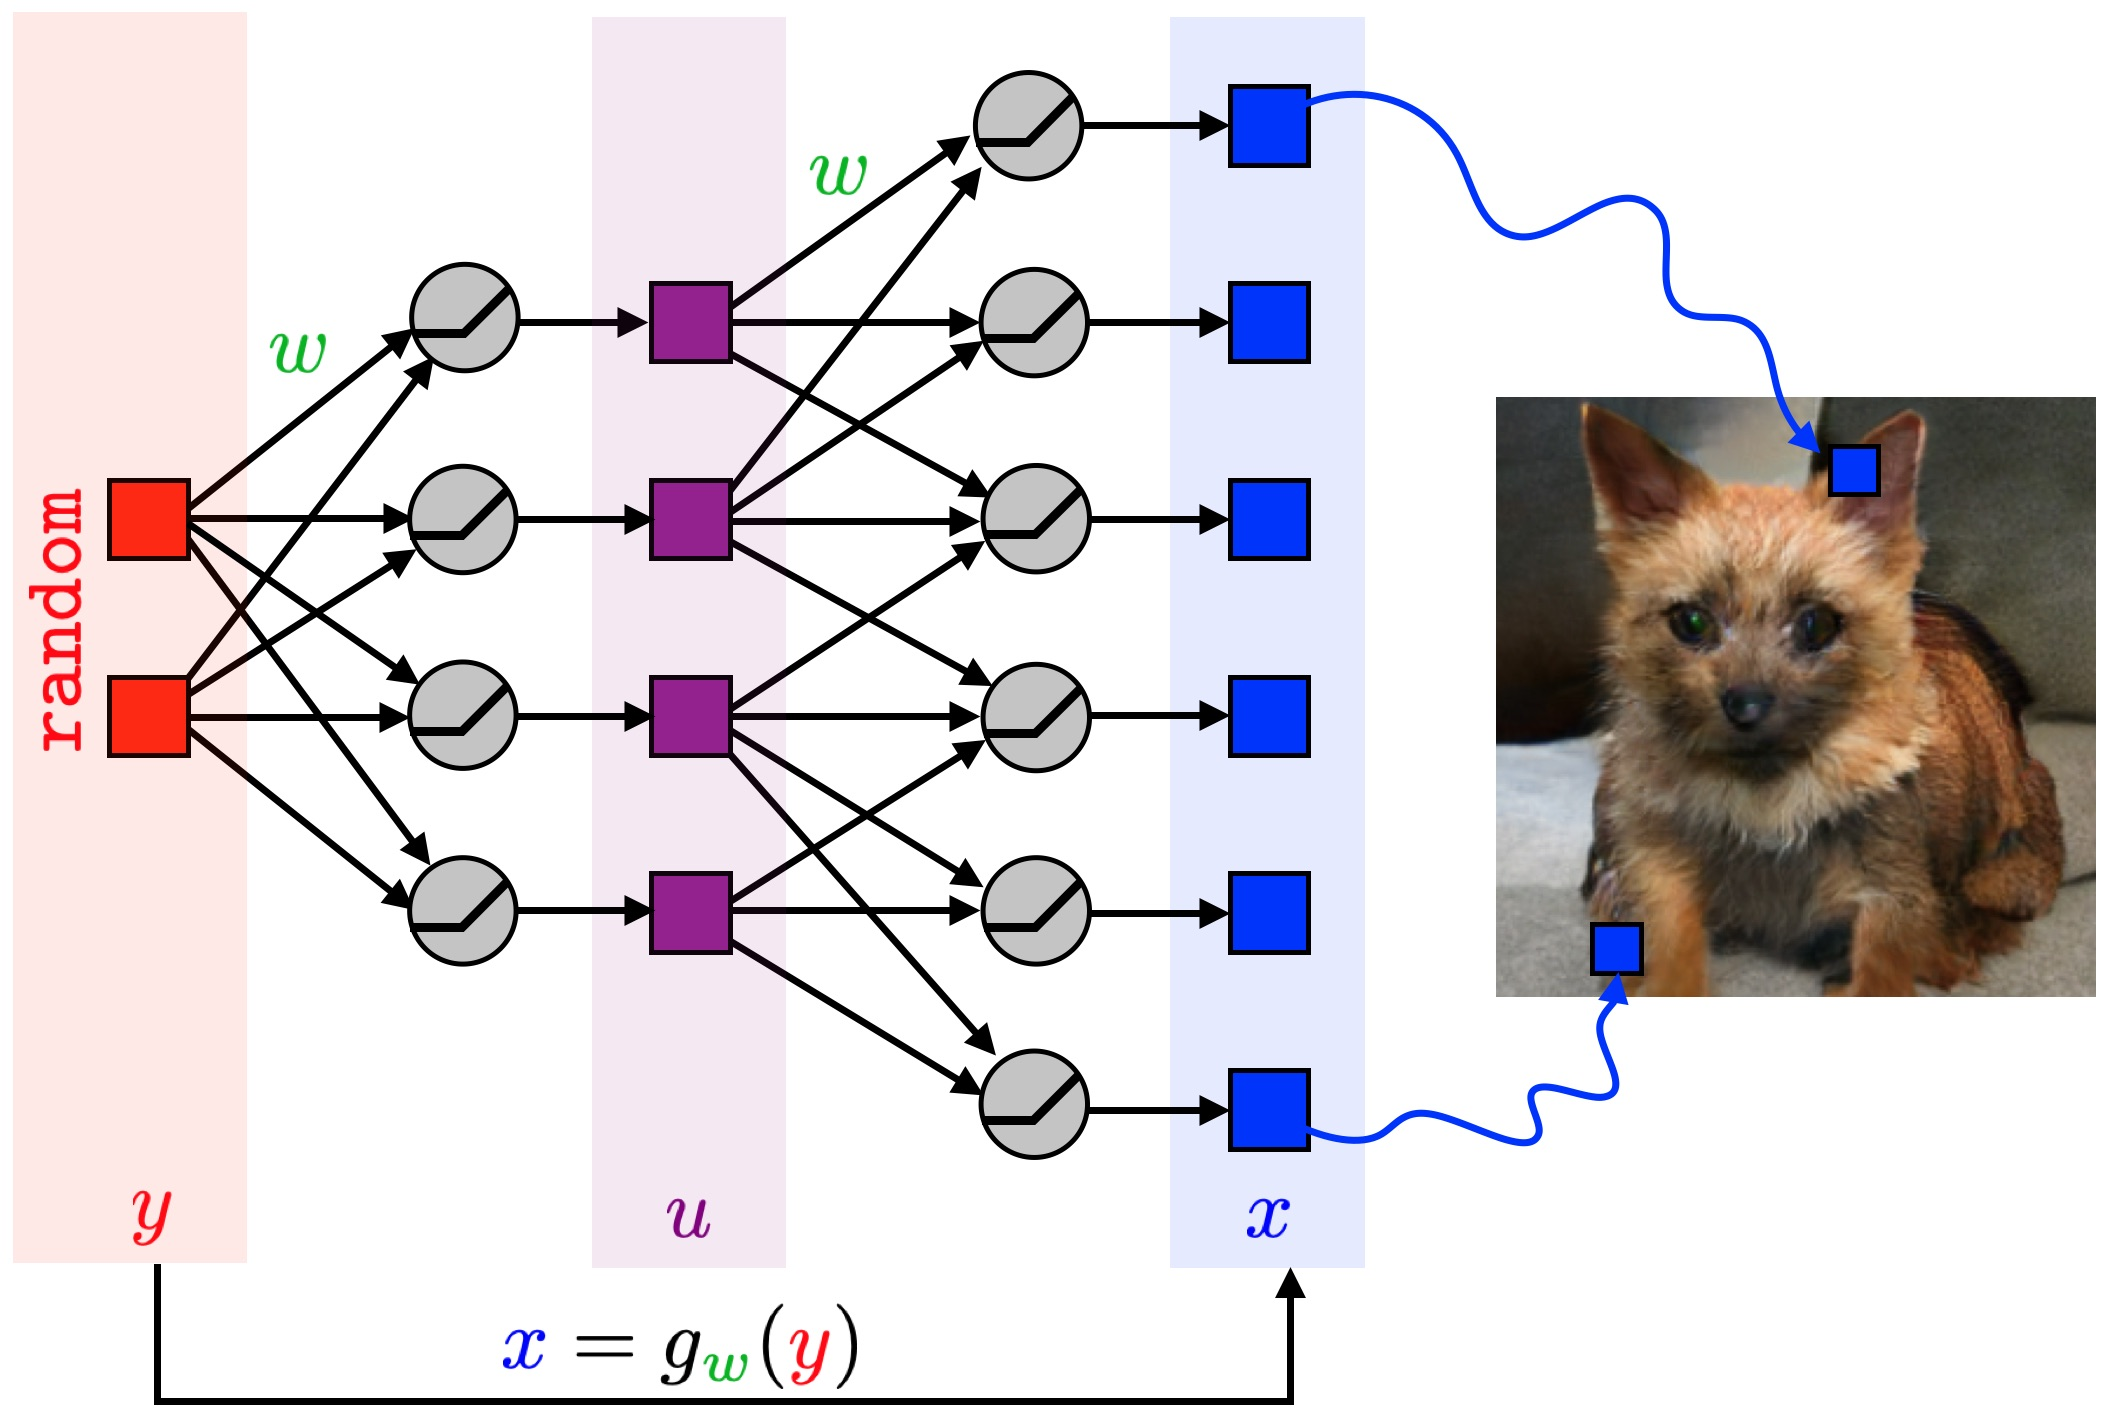
\includegraphics[width=.82\linewidth]{generative-en.jpg}
\caption{A schematic generator maps a random input $y$ through a hidden layer to an image $x=g_w(y)$. Practical image generators have more layers and a much larger output dimension.}\label{fig:generative}
\end{figure}

For unconditional generation, training can use images without class labels. Their collection, selection, and preprocessing still require care. Conditional generation additionally supplies information such as a class label, giving a model $g_w(y,c)$. Thus not every generative model is trained without supervision.

The aim is to reproduce a distribution, including its diversity. If the reference distribution assigns probability $1/2$ to cats and $1/2$ to dogs, an ideal generator has those probabilities too. A finite random batch need not contain exactly half of each. A model that produces the same plausible image repeatedly has not learned the full distribution; this is an extreme form of mode collapse.

\subsection{Comparing empirical distributions}
\label{sec-app-gen}
Let $z_1,\ldots,z_n$ be training images, and let $x_i=g_w(y_i)$ be generated images from independent latent samples. Their empirical distributions are
\[
 \mu_{w,n}=\frac1n\sum_{i=1}^n\delta_{x_i},\qquad
 \nu_n=\frac1n\sum_{j=1}^n\delta_{z_j}.
\]
Using measures retains frequencies and repeated samples, which ordinary set notation would discard. One possible objective is a transport distance between these measures.

For Euclidean ground cost, the empirical Wasserstein distance of order one is
\begin{equation}\label{eq-nn-w1}
 W_1(\mu_{w,n},\nu_n)
 =\frac1n\min_{s\in\Sigma_n}\sum_{i=1}^n\norm{g_w(y_i)-z_{s(i)}}_2.
\end{equation}
The factor $1/n$ normalizes the total probability mass. This distance is different from the squared quadratic cost introduced in the transport chapter. For unequal sample counts or weights, replace the permutation by a coupling with the prescribed marginals.

\begin{figure}[htbp]\centering
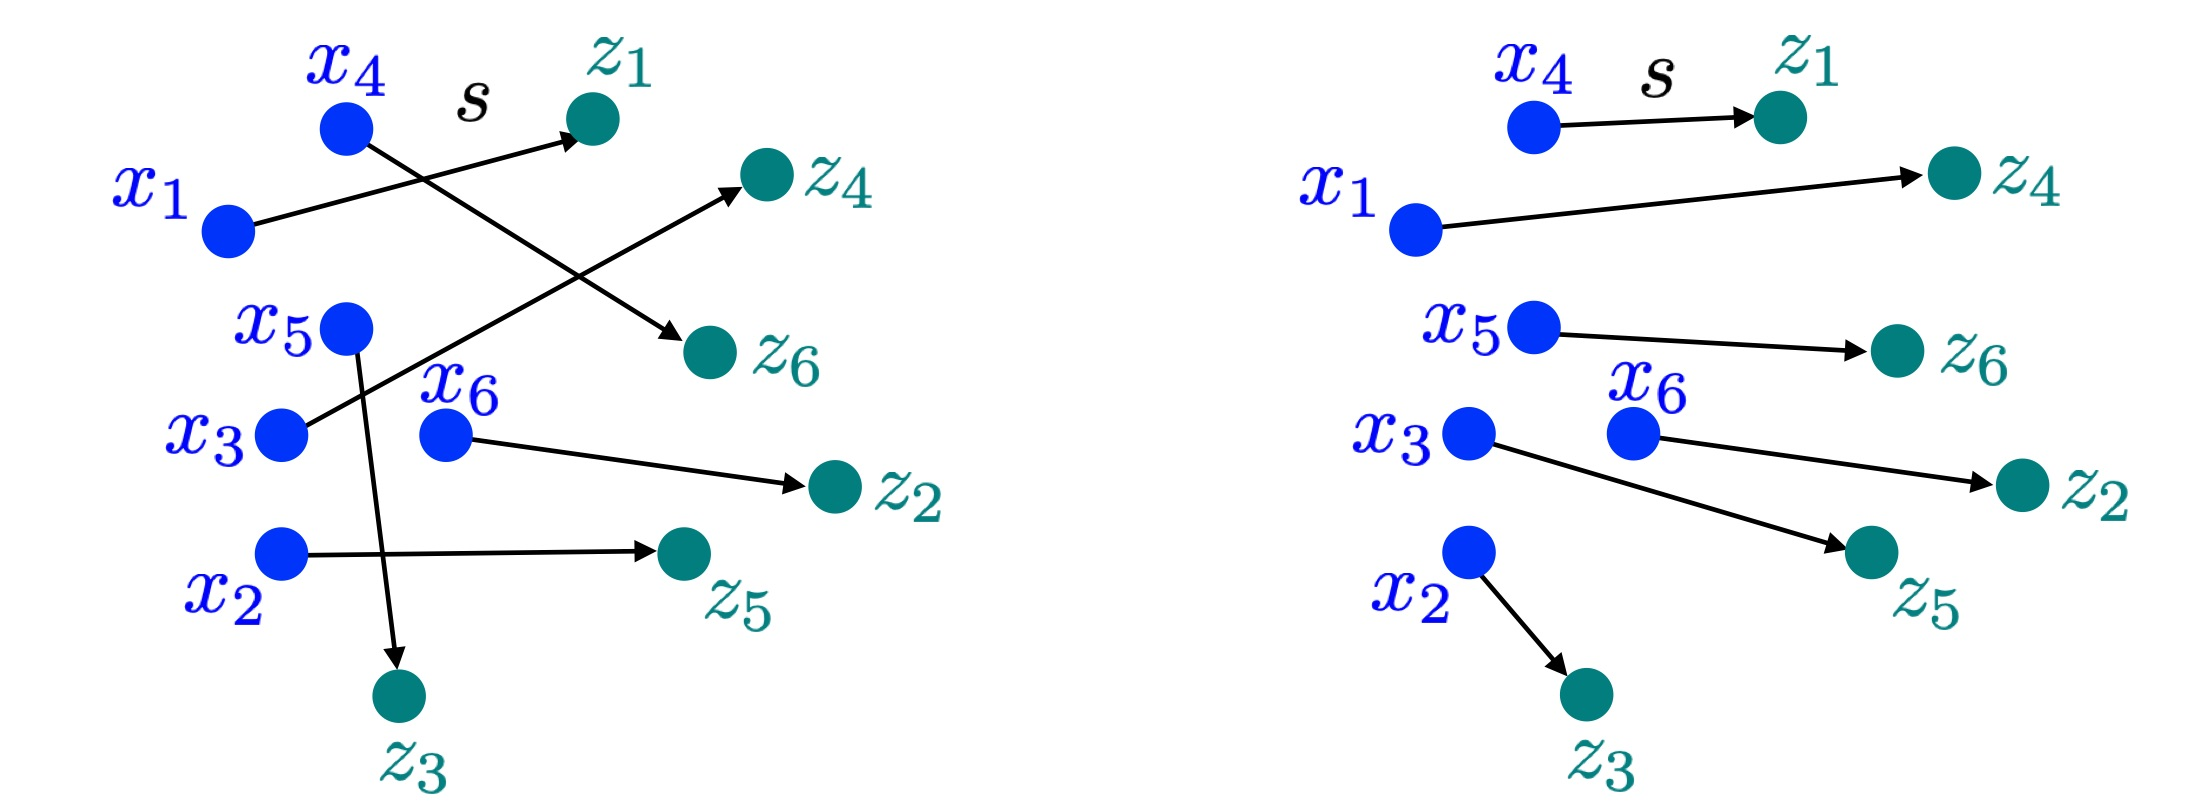
\includegraphics[width=.84\linewidth]{otmonge.jpg}
\caption{Two assignments of six source points to six target points. The right-hand assignment has smaller Euclidean transport cost and is the optimal matching in this example.}\label{fig:otmonge}
\end{figure}

In Figure~\ref{fig:otmonge}, the left assignment is $(1,5,4,6,3,2)$, while the optimal one on the right is $(4,3,5,1,6,2)$. The notation lists $(s(1),\ldots,s(6))$. Although there are $6!=720$ possibilities, efficient assignment algorithms avoid enumerating all $n!$ permutations and can solve a dense problem in $O(n^3)$ operations. The transport chapter explains the convex relaxation behind this computation~\cite{PeyreCuturi}.

The distributional learning objective is $\min_w W_1(\mu_w,\nu)$ for a target law $\nu$. Finite-sample transport provides a numerical approximation, but brings statistical and optimization difficulties. Transport between small batches is generally a biased estimate of the population distance. The optimal assignment may change as $w$ changes, so the empirical objective is not everywhere differentiable.

The ground distance also matters. Euclidean distance between pixel arrays is sensitive to small translations and may poorly reflect semantic similarity. A feature representation can provide a more relevant cost, but its choice changes the geometry being learned.

\subsection{Generative adversarial networks}
Generative adversarial networks (GANs), introduced by Goodfellow and collaborators in 2014~\cite{goodfellow2014generative}, train a generator against a discriminator. The discriminator $D_v(x)\in(0,1)$ tries to distinguish data from generated samples. The original minimax objective is
\begin{equation}\label{eq-gan}
 \min_w\max_v\left\{
 \mathbb E_{Z\sim\nu}[\log D_v(Z)]
 +\mathbb E_{Y\sim\eta}[\log(1-D_v(g_w(Y)))]\right\}.
\end{equation}
The discriminator increases the objective; the generator decreases it. Alternating gradient updates approximate this game, without a general guarantee of convergence for arbitrary networks.

For an unrestricted discriminator optimized exactly, the inner supremum equals $-\log4+2\operatorname{JS}(\nu,\mu_w)$, where the Jensen--Shannon divergence is
\[
 \operatorname{JS}(\nu,\mu)=\tfrac12\operatorname{KL}(\nu\mid m)
 +\tfrac12\operatorname{KL}(\mu\mid m),\qquad m=\tfrac12(\nu+\mu).
\]
Here KL uses natural logarithms and is defined between measures by their Radon--Nikodym densities. Both measures are absolutely continuous with respect to $m$. This identity concerns the ideal discriminator optimum; finite networks and incomplete optimization change the objective actually achieved. In practice, a commonly used generator loss is $-\mathbb E\log D_v(g_w(Y))$, which has the same desired distributional optimum but different gradients.

\subsection{The Wasserstein connection}
Wasserstein GANs~\cite{martin2017wasserstein} use a different objective, based on the Kantorovich--Rubinstein dual formula. For probability measures on $\RR^d$ with finite first moments,
\begin{equation}\label{eq-wgan-dual}
 W_1(\nu,\mu_w)=\sup_{\operatorname{Lip}(h)\le1}
 \left\{\mathbb E_{Z\sim\nu}h(Z)-\mathbb E_{Y\sim\eta}h(g_w(Y))\right\}.
\end{equation}
The constraint means $|h(x)-h(x')|\le\norm{x-x'}_2$ for all $x,x'$. A critic network approximates this class of functions, and its values are real scores, not class probabilities. The generator minimizes the discrepancy estimated by the critic.

The critic is a dual potential for a \emph{fixed} ground distance; it does not automatically learn a new transport cost between pairs of images. Enforcing or approximating the Lipschitz constraint is essential. Restricting the critic class and optimizing it only approximately also means that the computed score need not equal the true Wasserstein distance.

Ordinary GANs and Wasserstein GANs thus express related adversarial principles with different mathematical objectives. Neither training procedure guarantees that every generated image is meaningful or that all modes are represented.

\begin{figure}[htbp]\centering
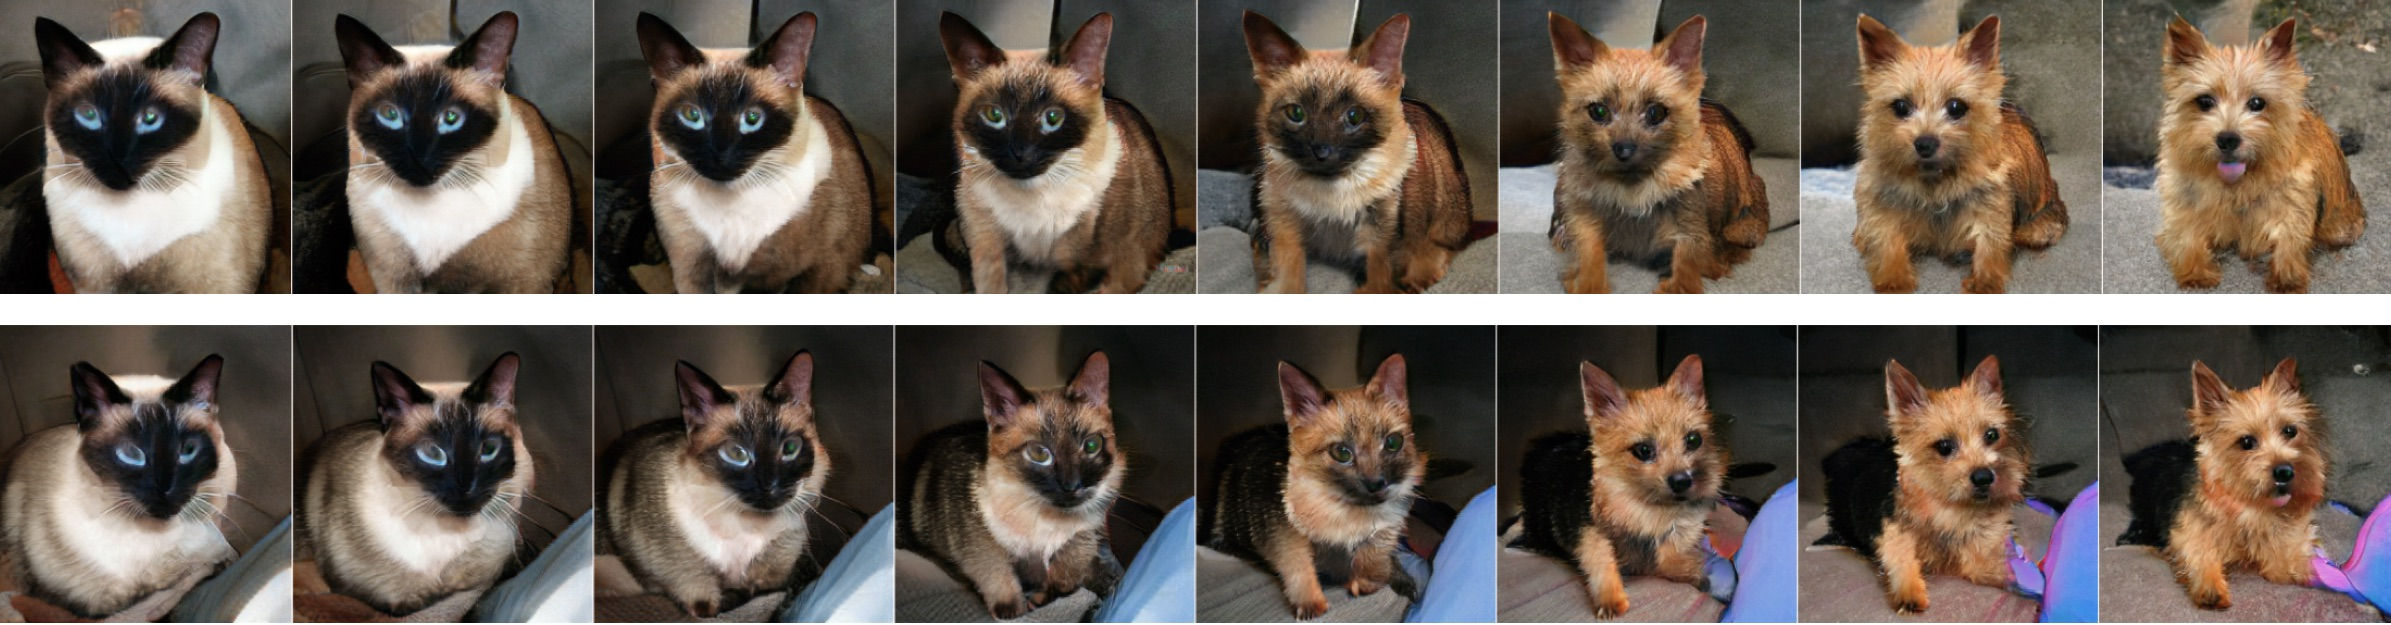
\includegraphics[width=.97\linewidth]{deepfake.jpg}
\caption{Two sequences of synthetic images interpolating between cats and dogs, using the BigGAN model~\cite{brock2018large}. BigGAN is class-conditional; its class information is part of the conditioning. These examples illustrate generation and interpolation rather than a claim of an optimal transport path.}\label{fig:deepfake}
\end{figure}

Interpolating latent or conditioning variables can produce smooth visual transitions, as in Figure~\ref{fig:deepfake}. Such paths need not be transport geodesics or remain typical under the training distribution. Visual plausibility, diversity, fidelity to the target distribution, and performance on held-out data are separate aspects of a generative model's quality.
